\documentclass[10pt]{article}
\usepackage{icmlko}

\icmlmeta{IP 파운데이션 월드모델}{118}{좋아함은 잘 재지는데}{다른 플랫폼에서 평점을 2,892건 이어 붙였다 --- 두 플랫폼 평점이 $\rho{=}+$0.969로 일치하는데(라벨은 $+$0.555) 전이는 $-$0.0005다}

\begin{document}

\twocolumn[
\icmlheader

\begin{abstract}
노트 117의 교훈은 ``평점은 물리량이 다르지만 \emph{같은 플랫폼}이라 절반만
다르다''였다. \textbf{다른 플랫폼의 다른 계수기}를 찾았다. MyAnimeList(Jikan)는
504로 막혀 있었고 \textbf{Kitsu} 가 열려 있었다. AniList \texttt{idMal} 4,716건을
다리로 세계애니 \textbf{2,892건(98\%)}을 이었다. 누수 규칙을 지켜 골랐다 ---
\texttt{userCount} · \texttt{favoritesCount} · \texttt{popularityRank} 는 라벨과
같은 물리량이라 안 쓰고 \texttt{averageRating} · \texttt{ratingRank} 만 썼다.
\textbf{채택 0이다} --- Kitsu 평점 $-$0.0005 · Kitsu 순위 $-$0.0005 · 두 플랫폼
평균 $-$0.0002, 전부 0 근처 보류다. \textbf{대신 새 수치가 나왔다.} 두 플랫폼의
평점이 \textbf{$\rho{=}+$0.969}로 일치한다($n{=}2{,}864$). 노트 79 · 83이 두
플랫폼 \emph{라벨}로 잰 것은 $+$0.555였다. 신뢰도 천장으로 바꾸면 \textbf{라벨
0.734 대 평점 0.984}다. \textbf{시끄러운 것은 축이 아니라 라벨이었다.} 그리고
여기서 이 프로젝트가 오래 피해 온 사실이 드러난다 --- \textbf{평점은 거의
완벽하게 재지는데도 전이를 못 돕는다.} 사람들이 무엇을 \emph{좋아하는지}는
두 플랫폼이 똑같이 말해 주는데, 그것이 얼마나 \emph{많이 볼지}를 안 알려 준다.
노트 93이 ``축에 없는 것 0.256''이라 부른 것의 일부는 \textbf{원리적으로 축에
담길 수 없는 것}이다 --- 질과 양은 다른 축이고, 질을 아무리 잘 재도 양이
안 나온다.
\end{abstract}
]

\begin{figure*}[t]
\centering
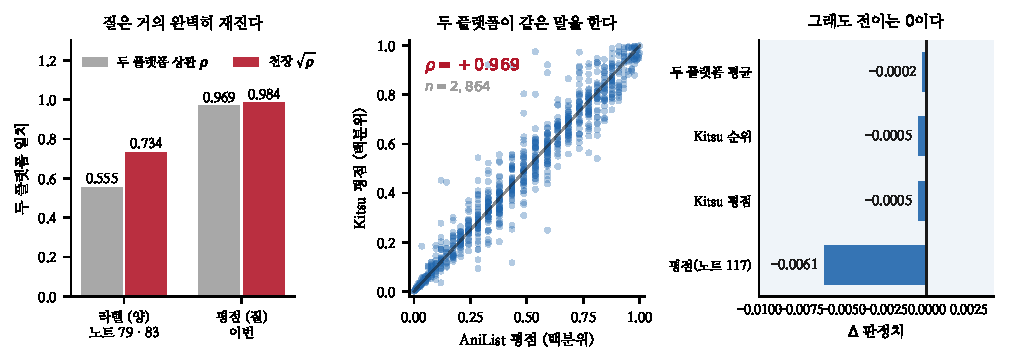
\includegraphics[width=\textwidth]{figs/ql.pdf}
\caption{왼쪽 --- 질은 거의 완벽히 재진다. 가운데 --- 두 플랫폼이 같은 말을
한다. 오른쪽 --- 그래도 전이는 0이다.}
\end{figure*}

\section{다른 플랫폼을 찾았다}

\begin{table}[t]
\centering\tsize
\caption{후보 셋을 두드렸다.}
\begin{tabular}{ll}
\toprule
MyAnimeList(Jikan) & \textbf{504 Gateway Time-out} \\
Kitsu & \textbf{열려 있다} \\
스팀 메타크리틱 & 덮개율 31\%(캐시) \\
\bottomrule
\end{tabular}
\end{table}

Kitsu 는 MAL 대응을 주므로 AniList \texttt{idMal} 을 다리로 쓸 수 있다.
스무 개씩 묶어 148번 요청, 148/148 성공, \textbf{세계애니 2,892/2,945(98\%)}.

\begin{table}[t]
\centering\tsize
\caption{Kitsu 에서 받은 것과 쓴 것.}
\begin{tabular}{lll}
\toprule
\texttt{averageRating} & \textbf{쓴다} & 다른 사용자층의 질 \\
\texttt{ratingRank} & \textbf{쓴다} & 그 순위 \\
\midrule
\texttt{userCount} & 안 쓴다 & 라벨과 같은 물리량 \\
\texttt{favoritesCount} & 안 쓴다 & 〃 \\
\texttt{popularityRank} & 안 쓴다 & 〃 \\
\bottomrule
\end{tabular}
\end{table}

노트 117의 출처 차단을 스스로에게 먼저 적용했다 --- 셋은 긁어 두고 안 썼다.

\section{채택 0}

\begin{table}[t]
\centering\tsize
\caption{전수 검정 24개 · 422초. 평점 계열만.}
\begin{tabular}{lrrl}
\toprule
& $\Delta$ & 채택 & 구간(첫 씨앗) \\
\midrule
두 플랫폼 평균 & $-$0.0002 & 0/4 & $-$0.0036 $\sim$ $+$0.0061 \\
Kitsu 순위 & $-$0.0005 & 0/4 & $-$0.0037 $\sim$ $+$0.0062 \\
Kitsu 평점 & $-$0.0005 & 0/4 & $-$0.0037 $\sim$ $+$0.0062 \\
평점(노트 117) & $-$0.0061 & 0/4 & $-$0.0189 $\sim$ $+$0.0030 \\
\bottomrule
\end{tabular}
\end{table}

구간이 매우 좁다($\pm$0.005). \textbf{못 넘는 것이 아니라 아무 일도 안
일어난다.}

\section{그런데 질은 거의 완벽히 재진다}

\begin{table}[t]
\centering\tsize
\caption{두 플랫폼이 같은 것을 잴 때 얼마나 맞나.}
\begin{tabular}{llrr}
\toprule
& 무엇을 & $\rho$ & 천장 $\sqrt{\rho}$ \\
\midrule
노트 79 · 83 & 라벨(양) & $+$0.555 & \textbf{0.734} \\
\textbf{이번} & \textbf{평점(질)} & \textbf{$+$0.969} & \textbf{0.984} \\
\bottomrule
\end{tabular}
\end{table}

AniList 와 Kitsu 는 다른 사이트, 다른 사용자층, 다른 평점 눈금(100점 대 100점)을
쓴다. 그런데 2,864건에서 순위 상관이 \textbf{$+$0.969}다.

\claimx{\textbf{시끄러운 것은 축이 아니라 라벨이다.} 같은 두 플랫폼 구조에서
질은 $+$0.969로 맞고 양은 $+$0.555로 맞는다. 노트 83의 라벨 천장 0.734는
\emph{양}을 재는 것이 어렵다는 뜻이지 세상이 예측 불가라는 뜻이 아니다.}
{세계애니 하나에서 쟀다. 노트 79 · 83은 웹툰/만화와 애니/세계애니 두 쌍에서
$+$0.52$\sim+$0.56을 얻었으므로 라벨 쪽은 두 번 확인됐지만 평점 쪽은
한 번이다.}

\section{질과 양은 다른 축이다}

\begin{quote}\fontsize{9.5}{11.5}\selectfont
\textbf{평점은 거의 완벽하게 재지는데도 전이를 못 돕는다}($\Delta-$0.0005,
구간 $\pm$0.005). 사람들이 무엇을 \emph{좋아하는지}는 두 플랫폼이 똑같이
말해 주는데, 그것이 얼마나 \emph{많이 볼지}를 안 알려 준다.
\end{quote}

\claimx{노트 93이 ``축에 없는 것 0.256''이라 부른 것의 일부는 \textbf{원리적으로
축에 담길 수 없는 것}이다. 질을 아무리 잘 재도 양이 안 나온다 --- 측정 잡음
때문이 아니라 두 물리량이 다르기 때문이다.}{``전이를 못 돕는다''는 이 구조에서
그렇다는 뜻이다. 라벨을 질로 바꾸면(예: 팝업 만족도) 평점 축이 크게 도울
것이다. \textbf{다만 사업이 묻는 것은 몇 명 오는가이지 얼마나 좋았는가가
아니다.}}

\begin{table}[t]
\centering\tsize
\caption{이 프로젝트가 재는 것.}
\begin{tabular}{lll}
\toprule
& 물리량 & 두 플랫폼 일치 \\
\midrule
라벨 & \textbf{양}(방문자 · 리뷰 수 · 후원자) & $+$0.555 \\
새 축 후보 & 질(평점) & $+$0.969 \\
\midrule
\multicolumn{3}{l}{\textbf{둘의 관계 --- 세계애니에서 $\rho{=}+$0.41}} \\
\bottomrule
\end{tabular}
\end{table}

질과 양의 상관이 $+$0.41이다. 겹치는 것이 17\%뿐이므로 질을 완벽히 알아도
양의 83\%는 여전히 모른다.

\section{한계}

\begin{itemize}[leftmargin=1.1em,itemsep=0.15em]
\item \textbf{채택할 것이 없다.} 평점 계열 넷이 전부 0 근처다.
\item 평점 천장 0.984를 세계애니 하나에서 쟀다.
\item Kitsu 를 세계애니에만 붙였다. 만화도 idMal 이 있는데 Kitsu 의 만화
      대응은 안 봤다.
\item ``질이 양을 안 설명한다''를 상관 $+$0.41 하나로 말했다. 도메인마다
      다를 수 있다.
\item 스팀 메타크리틱(전문가 평점)은 덮개율 31\%라 안 넣었다. 그것은
      \emph{사용자}가 아니라 \emph{비평가}라 또 다른 계수기다.
\end{itemize}

\section{다음}

\begin{enumerate}[leftmargin=1.3em,itemsep=0.15em]
\item \textbf{양을 재는 다른 계수기} --- 질은 막혔다. 양을 \emph{다른
      플랫폼}에서 재면 라벨 잡음을 줄일 수 있다(노트 83의 천장을 올리는 길).
      Kitsu \texttt{userCount} 를 축이 아니라 \textbf{라벨 보정}에 쓴다 ---
      두 플랫폼 평균이 참값에 더 가깝다.
\item \textbf{팝업 레코드} --- 열두 노트가 같은 곳을 가리킨다.
\item 만화에도 Kitsu 를 붙인다.
\item 텀블벅 API --- 펀딩만 미디어 홍보 0\%다.
\end{enumerate}

\vspace{0.6em}
\hrule height 0.3pt
\vspace{0.5em}
{\footnotesize
\textbf{참고문헌}\\[0.3em]
Lord, F. M., Novick, M. R. (1968). \emph{Statistical Theories of Mental Test
Scores}. Addison-Wesley.\\[0.15em]
Kaufman, S. et al. (2012). Leakage in data mining: formulation, detection, and
avoidance. \emph{ACM TKDD}, 6(4), 1--21.\\[0.15em]
Spearman, C. (1904). The proof and measurement of association between two
things. \emph{American Journal of Psychology}, 15(1), 72--101.\\[0.15em]
Ben-David, S. et al. (2010). A theory of learning from different domains.
\emph{Machine Learning}, 79(1--2), 151--175.\\[0.15em]
Efron, B., Tibshirani, R. J. (1993). \emph{An Introduction to the Bootstrap}.
Chapman \& Hall.
}

\end{document}
